\documentclass{article}
\usepackage{geometry}
\usepackage{graphicx}
\usepackage{hyperref}

\title{Design and Implementation of a Teleoperated Robot for Industrial Inspection, Repair, and Maintenance (IRM) Tasks}
\author{Lars Gielen \\ Vinz Roosen}
\date{\today}

\begin{document}
\maketitle

\section{Introduction}

Industrial facilities often require routine inspection, repair, and maintenance (IRM) tasks to ensure optimal operation and safety standards. However, performing these tasks manually can be hazardous and time-consuming. To address these challenges, this paper presents a teleoperated robot designed to execute IRM tasks in industrial environments. The teleoperation capability ensures human operators can remotely control the robot, mitigating safety risks associated with manual interventions.

\section{Design Requirements}
The design of the teleoperated robot for IRM tasks is guided by the following requirements:

\begin{itemize}
    \item Safety: Ensure the safety of operations in the industrial facility, preventing damage to equipment and minimizing risks to human operators.
    \item Teleoperation: Enable remote control of the robot via a web browser interface to facilitate device-agnostic operation.
    \item Sensor Suite: Equip the robot with sensors for environmental perception, object detection, and monitoring of critical parameters.
    \item Actuation Mechanisms: Implement actuators for manipulation, locomotion, and tool operation to perform diverse IRM tasks.
\end{itemize}

\newpage
\section{Hardware Components}

The teleoperated robot comprises the following hardware components:

\begin{itemize}
    \item Robotic Platform: A mobile base equipped with wheels for agile navigation in industrial environments. The robot used for this project is shown in Figure \ref{fig:turtlebot}.

        \begin{figure}[h]
        \centering
        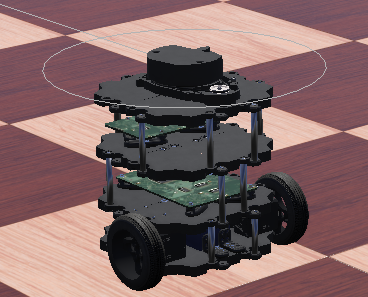
\includegraphics[width=0.5\linewidth]{Design Document/TurtleBot3.png}
        \caption{TurtleBot3 used for this project}
        \label{fig:turtlebot}
    \end{figure}
    
    \item Sensor Suite: Includes cameras, LiDAR, GPS and inertial measurement units (IMUs) for perception and environment monitoring.
    
    \item Communication System: Utilizes Wi-Fi or cellular connectivity for real-time communication between the robot and teleoperation interface. The communication is based around MQTT.
\end{itemize}

\section{Software Architecture}

The software architecture of the teleoperated robot consists of the following modules:

\begin{itemize}
    \item Perception: Processes sensor data to detect objects, and identify obstacles.
    \item Input: Receive input from browser user interface and pipe to Control Module.
    \item Control: Implements teleoperation commands to control the robot's motion and tool/sensor operations.
    \item Safety Monitoring: Monitors environmental conditions and robot status to prevent collisions, avoid hazards, and ensure safe operations.
    \item User Interface: A web-based interface for teleoperation, providing live video feeds, control buttons, and status indicators.
\end{itemize}

\subsection{Perception Module}
\begin{itemize}
    \item \textbf{Input:} Reading the sensor (LiDAR, Camera, GPS, etc.) data.
    \item \textbf{Computing:}
    \begin{itemize}
        \item Processing sensor data: Perform data filtering, segmentation, and feature extraction to identify objects and obstacles in the environment.
        \item Path planning: Calculate safe and efficient paths for the robot to navigate through the environment while avoiding obstacles detected by LiDAR.
        \item Object recognition: Analyze LiDAR data to recognize specific objects or structures relevant to the inspection, repair, or maintenance tasks.
        \item Determining the robot's relative location in working environment with GPS
    \end{itemize}
    \item \textbf{Output:}
    \begin{itemize}
        \item Navigation commands: Transmit motion commands to the robot's actuators.
        \item Visualization: Display processed LiDAR data, maps, and navigation information to the teleoperator through the browser interface.
        \item Alerts and notifications: Provide real-time feedback to the operator about detected obstacles, critical events, or safety concerns.
        \item Task execution feedback: Relay information about the progress of inspection, repair, or maintenance tasks performed by the robot.
    \end{itemize}
\end{itemize}

\subsection{Input Module}
The input module serves as the interface between the teleoperation interface accessed through a web browser and the robot's control system. Its primary function is to convert user input from the web browser into a standard format compatible with the robot's controller. This approach reduces coupling between the teleoperation interface and the robot's internal components, facilitating modularity and scalability.

\begin{itemize}
    \item \textbf{Parsing}: Analyzing the input stream to identify distinct commands or gestures. For example, separating keyboard strokes into individual commands or recognizing specific patterns in gesture data.
    \item \textbf{Validation}: Verifying the integrity and validity of the input data to ensure it conforms to expected formats and ranges. Invalid or malformed input is discarded or flagged for further action.
    \item \textbf{Normalization}: Standardizing input values to a common format or range suitable for the robot's control system. This may involve converting units, scaling values, or applying calibration factors to ensure consistent behavior across different input devices and operating conditions.
\end{itemize}
Once the input data is processed and validated, the input module generates output commands in a standardized format compatible with the robot's control system. These commands are transmitted to the controller via the communication system, enabling real-time control and supervision of the robot's actions. By decoupling the teleoperation interface from the underlying control logic, the input module promotes modular design principles and facilitates future enhancements or modifications to the system architecture.

\subsection{Control Module}
The Control Module serves as the central hub for overseeing and regulating the teleoperation of the robot, ensuring precise control, safety, and adaptability.
\begin{itemize}
    \item Receives input from an input component to control the actuators.
    \item Utilize PID controllers to maintain stability and accuracy during robot movements.
    \item Incorporates robust safety mechanisms to prevent accidents and safeguard both the robot and its surroundings.
\end{itemize}

\subsection{Safety Monitor}
\begin{itemize}
    \item Emergency stop buttons
    \item Collision detection system
    \item Collision avoidance algorithms
    \item Error detection and recovery mechanisms
    \item Redundant safety checks
\end{itemize}

\subsection{User Interface}
\begin{itemize}
    \item Intuitive controls for robot maneuvering
    \item web browser interface
    \begin{itemize}
        \item Front-end: HTML, CSS and JavaScript
        \item Local hosting
    \end{itemize}
    \item Controls for manipulator and tool operation
    \item Function activation buttons
    \item Real-time sensor data visualization
    \item Status indicators for robot condition and task progress
    \item Live video streaming from onboard cameras
\end{itemize}


\section{Teleoperation Mechanism}
The teleoperation mechanism allows human operators to remotely control the robot's actions through a web browser interface. Key features include:

\begin{itemize}
    \item Live Video Streaming: Provides real-time video feeds from onboard cameras, enabling operators to visualize the robot's surroundings.
    \item Control Interface: Offers intuitive controls for driving the robot, manipulating the arm, and activating tools.
    \begin{itemize}
        \item Keyboard Input
        \item Joystick Control
        \item Autonomous navigation
    \end{itemize}
    \item Safety Overrides: Incorporates emergency stop buttons and collision avoidance algorithms to prevent accidents and ensure safe operation.
    \item Feedback Mechanisms: Provides visual and auditory feedback to the operator, indicating the robot's status, battery level, and task completion.
\end{itemize}

\end{document}
